\documentclass[14pt]{extreport}
\usepackage{gost}
\usepackage{lscape}
\usepackage{lscape}
\usepackage[justification=centering]{caption}
\sloppy
\tolerance=500
\hyphenpenalty=10000
%Тут можно вставить дополнительные пакеты

\begin{document}
\pagestyle{empty} %  выключаем нумерацию

\includepdf[pages=-,pagecommand={}]{titulCourse.pdf}
\setstretch{1.5}
\pagestyle{plain} % включаем нумерацию

\tableofcontents
\intro 
    В современном мире все больше людей обращаются к веб-сервисам для %
    автоматизации и упрощения собственной жизни. Они органично вписались %
    во все направления жизни людей современного общества.  

    Одним из таких инструментов упрощения и автоматизации жизнедеятельности может %
    стать веб-приложение для составления графика лечения на основании рекомендаций %
    врача. Помимо удобства для пациентов, данное приложение может помочь докторам для %
    более эффективного контроля процесса лечения.

    Актуальность приложения обоснована следующим: по данным исследования Ассоциации директоров по коммуникациям и %
    корпоративным медиа России (АКМР)\cite{internet_users} от 2023 года показывает что 78 процентов %
    Россиян пользуются интернетом на регулярной основе, что показывает большой %
    охват аудитории для полноценной реализации и интеграции будущего веб-приложения.

    В дополнение к этому, с учетом увеличивающейся численности старшего поколения %
    и необходимости улучшения доступа к медицинским услугам, веб-приложение %
    подобного рода может иметь значительный потенциал для улучшения уровня %
    здравоохранения. Это также может помочь уменьшить нагрузку на медицинский %
    персонал, освободив их время для более критически важных задач. Кроме того, %
    с учетом текущей ситуации в мире, веб-приложения для здравоохранения открывают %
    новые возможности для дистанционного взаимодействия и контроля за процессом %
    лечения, что делает их еще более актуальными и востребованными.

    Целью данной практической работы является проектирование и разработка веб-приложения для составления графика лечения на %
    основании рекомендаций врача.

    Из составленной цели были выдвинуты следующие задачи:
        \begin{itemize}
            \item Анализ конкурентов и аналогов приложения;
            \item Составление функциональных и не функциональных требований;
            \item Разработка базы данных прилоежения;
            \item Составление диаграм взаимодействия пользователей с системой;
            \item Выбор технологий программирования для создания конечного продукта;
            \item Анализ бизнес требоавний к приложению;
        \end{itemize}

\chapter{Сравнение аналогов проектируемой системы}
    В ходе тщательного анализа и изучения предметной области, %
    мы провели обширный поиск и исследовали существующие аналоги %
    на рынке. Данное исследование включало в себя изучение различных приложений и %
    сервисов, их функционала, возможностей и особенностей. %
    В результате, мы смогли выявить ряд ключевых аналогов, %
    которые в настоящее время существуют и активно используются. %
    Эти аналоги представляют собой различные продукты и решения, %
    которые в той или иной степени могут совпадать с нашими целями %
    и задачами. Изучение этих аналогов помогает нам лучше понять %
    существующий рынок, определить ключевые тренды и возможности для %
    инноваций. Изученные аналоги изображены в таблице 1.1.
    
    \newpage
    \begin{landscape}
        
        \begin{table}[]
            \label{analogs}
            \caption{Таблица сравнения аналогов}
            \resizebox{\columnwidth}{!}{%
            \begin{tabular}{|p{9em}|p{13em}|p{9em}|p{10em}|p{9em}|}
            
            \hline
            Название Аналога & Возможности & Тариф & Достоинства & Недостатки \\
            \hline
            1 & 2 & 3 & 4 & 5 \\
            \hline
            Medisafe & Мобильное приложение, которое помогает отслеживать приём лекарств по дате и времени приёма с примечанием. Также существует интеграция с приложением хранящим и обновляющим данные о здоровье и есть возможность составлять отчёт о приёме. & Бесплатное досупны базовые функции, остальные как кастомизация уведомлений и внешнего вида и отсутсвие рекламы доступны по подписке 4.99\$ в месяц и 39.99\$ в год. & Возможность следить за приёмом лекарств членов семьи и создание отчётности о лечении. Присутсвие примечения о способе приёма лекарства и дозировки. Интерграция с приложением следящим за показателями здоровья. & Система уведомлений не гибкая и не настраиваемая. \\
            \hline
            Mytherapy & Мобильное приложение, которое напоминает о приёме лекарств, отслеживает показатели здоровья и имеет возможность создания отчётов приёме. & Бесплатное приложение & Существование журнала о пропущенных и подтверждённых приёмов лекарств. Отслеживание оставшегося количсетва лекарств. Поддержка схем дозировок. Выбор измерений показателей взависимости от заболевания. Семейный доступ к приёму лекарств. & Обязует следить за количеством лекарств. Не удобный выбор временит приёма. \\
            \hline
        \end{tabular}%
            }
            \end{table}
        
        \newpage

        \begin{table}[]
            \begin{flushright}
                Продолжение таблицы 1.1
            \end{flushright}
            \resizebox{\columnwidth}{!}{%
            \begin{tabular}{|p{9em}|p{13em}|p{9em}|p{10em}|p{9em}|}
            \hline
            1 & 2 & 3 & 4 & 5 \\
            \hline
            Мои таблетки & Мобильное приложение напоминающее о приёме лекарств. Так же имеющие возможность хранить историю приёмов. И создавать примечание о приёме. & Бесплатно доступно 10 курсов приёмов лекарств. По подписке 1.99\$ в месяц доступно неограниченное количество курсов приёмов. & Гибкая система уведомлений. Архив приёмов лекарств. & Отсутсвие семейнного доступа и учёта пропущенных приёмов. \\
            \hline
            Mr.Pillster & Мобильное приложение напоминающие о приёме лекарств и о измерении данных о здоровье. Существует возможность создавать график приёмов и измерений. Семейный доступ к приёмам лекарств. Быстрые кнопки “принять” и “отложить” в пуш-уведомлении & Бесплатно доступно добавление только прёмов лекарств. По подписке 329 рублей раз в три месяца, 749 рублей в год и 1790 рублей единоразово доступны все функции. & Возможность создать напоминание о измерении данных о здоровье. Семейный доступ к приёму лекарств. Возможность отложить приём лекарства при появлении уведомления. & В сравнение с другими приложениями не полный список типов дозировок. Также отсутсвие возможности создать собственное примечание к приёму лекарства. \\
            \hline
            Pills time & Мобильное для напоминаний о приёме лекарств и приёмах к врачу. Семейный доступ к приёмам. Возможность добавить фото к добавленному лекарству. Гибкий выбор периодичности приёма. & Бесплатное добавление курса лекарств, без. По подписке 99 рублей в месяц в год будут доступны все функции. & Большой список примечаний связанных с едой. Семейный доступ. Возможность создать расписание приёмов у врача. & Неудобная система уведомлений. Короткий список типов дозировок. \\
            \hline 
        \end{tabular}%
            }
            \end{table}
        
    \end{landscape}%
    
\chapter{Анализ функицональных и нефукциональных требований}
    В данной главе будет представлен анализ будущего приложения %
    с точки зрения выделения функциональных и нефукциональных требований.
    \section{Функциональные требования}
        В процессе анализа требований к веб-приложению для %
        составления графика лечения на основе рекомендаций врача были выделены %
        следующие фукнциональные требовация, которые необходимы для полноценного %
        функционирования приложения:
        \newline
        \begin{enumerate}
            \item Веб-приложение должно позволять пациенту или его %
            лечащему врачу создавать график лечения на основании %
            рекомендаций и назначений. Для этого необходимо предоставить %
            пользователю возможность добавлять информацию о лекарствах, %
            дозах и промежутках времени приема, а также продолжительность %
            лечения. График должен быть составлен на необходимый период %
            времени и сохраняться для каждого пациента.
            
            \item Приложение должно иметь функцию добавления %
            рекомендаций и назначений, включая лекарства, %
            дозы и промежутки времени приема.

            \item Приложение должно позволять врачу указывать %
            продолжительность лечения, чтобы график был составлен %
            на необходимый период времени.

            \item Приложение должно предоставлять возможность %
            сохранять и редактировать график лечения для каждого %
            пациента, чтобы врач мог обновлять его при необходимости.

            \item Приложение должно иметь функцию проверки наличия %
            противопоказаний и взаимодействия между различными %
            лекарствами, чтобы врач мог быть уверен в безопасности %
            назначенного лечения.

            \item Приложение должно предоставлять возможность %
            врачу проверить, были ли выполнены назначения пациентом, %
            путем отметки о выполнении каждой рекомендации.

            \item Приложение должно создавать напоминания для пациента %
            о приеме лекарств и выполнении других назначений, %
            которые были добавлены самим пациентом или его лечащим врачом.

            \item Приложение должно обеспечивать безопасное хранение %
            конфиденциальной информации о пациентах и доступ только %
            для авторизованных врачей.
        \end{enumerate}

    \section{Нефункциональные требования}

        После формулироваиня функицональных требований к системе и анализа %
        системы с точки зрения взаимодействия с конечным потребителем, были выделены %
        следующие нефункциональные требования:
        \newline
        \begin{enumerate}
            \item Веб-приложение должно иметь интуитивно понятный и %
            привлекательный интерфейс для пользователей всех возрастов %
            и уровней навыков. 

            \item Приложение должно поддерживать различные устройства и %
            разрешения экранов, включая мобильные устройства, планшеты %
            и компьютеры. 

            \item Гарантия конфиденциальности и безопасности %
            персональных медицинских данных пациентов. Так как данный аспект %
            строго регулируется государством. 

            \item Обеспечить совместимость с различными современными бразуерми, %
            при помощи который будет исполняться взаимодействие с приложением для %
            удобства пользователей

            \item Обеспечить быструю загрузку и отзывчивость интерфейса %
            при работе с графиком лечения и рекомендациями врача.

            \item Поддерживать возможность локализации интерфейса на %
            русском языке для удовлетворения потребностей пользователей %
            на территории Российской федерации.

            \item Реализовать авторизацию и управление доступом к %
            приложению и данным для обеспечения безопасности и %
            ограничения доступа к конфиденциальным данным.

            \item Обеспечить отказоустойчивость для минимизации времени %
            простоя и потери данных в случае сбоев или неполадок. %
            Приложение должно быть обеспечено необходимыми механизмами %
            для минимизации времени простоя и потери данных в случае %
            возникновения сбоев или неполадок. Это означает, что %
            система должна быть способна восстанавливаться после %
            сбоев без значительного воздействия на функциональность и производительность, обеспечивая непрерывность предоставления услуг пользователям.
        \end{enumerate}

\chapter{Диаграммы прецедентов}
    В данном разделе будут представлены взаимодействия основных пользователей %
    и ролей в системе в виде диаграмм прецедентов и схем активности. Для создания %
    изображений диаграмм было использовано бесплатное программное обеспечения под названием %
    "diagrams.net".\ \cite{diagrams_dot_net} %
    
    \section{Диаграмма прецедентов для сущности "Пользователь"\ }
        Сущность "Пациент"\ имеет следующие возможности:
        \begin{enumerate}
            \item Добавить прием лекарства: Эта возможность позволяет пациенту добавить %
            информацию о приеме лекарства. В процессе добавления создается уведомление, %
            которое отправляется пациенту телеграмм-ботом в определенное время, заданное пациентом;
            \item Добавить визит врача: Эта возможность позволяет пациенту добавить информацию о %
            визите к врачу. В процессе добавления создается уведомление, которое отправляется пациенту %
            телеграмм-ботом в определенное время, заданное пациентом;
            \item Регистрация пациента: Эта возможность позволяет пациенту зарегистрироваться в системе. %
            В процессе регистрации создается экземпляр пациента в базе данных;
            \item Редактирование профиля: Эта возможность позволяет пациенту редактировать свои данные в %
            профиле. В процессе редактирования обновляются данные в базе данных;
            \item Отправка обратной связи: Эта возможность позволяет пациенту отправить обратную связь о системе %
            или услугах. В процессе отправки обновляются данные в базе данных;
        \end{enumerate}
        
        Таким образом, сущность "Пациент"\ имеет пять возможностей, некоторые из которых %
        включают в себя создание уведомления и их отправку телеграмм-ботом, а также обновление %
        данных в базе данных. Диаграмма сущностей изображена на рисунке \ref{patient_uml}.

        \begin{figure}[H]%current location
            \centering
            \scalebox{0.75}{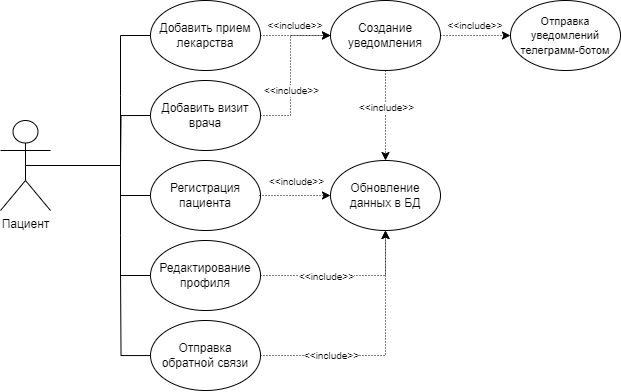
\includegraphics{pics/UML/Patient.png}}
            \caption{Диаграмма прецедентов для роли "Пациент".} \label{patient_uml}
        \end{figure} 
    
    \section{Диаграмма прецедентов для сущности "Доктор"\ }
        Сущность "Доктор"\ имеет следующие возможности:
        \begin{enumerate}
            \item Добавить график лечения пациентов: Эта возможность %
            позволяет доктору добавлять информацию о приемах лекарств %
            для пациента. В процессе добавления создается уведомление, %
            которое отправляется пациенту телеграмм-ботом в определенное %
            время, заданное доктором;
            \item Назначить прием: Эта возможность позволяет доктору %
            назначить прием с пациентом. В процессе добавления создается %
            уведомление, которое отправляется пациенту телеграмм-ботом в %
            определенное время, заданное доктором;
            \item Регистрация доктора: Эта возможность позволяет доктору %
            отправить заявку на регистрацию модератору веб-приложения. %
            В процессе регистрации создается экземпляр доктора с %
            атрибутом active=False и заявка на подтверждение данных %
            для модератора в базе данных;
            \item Редактирование профиля: Эта возможность позволяет доктору %
            редактировать свои данные в профиле. В процессе редактирования %
            обновляются данные в базе данных;
            \item Получить список пациентов: Эта возможность позволяет доктору %
            получить список лечащихся и уже прошедших лечение пациентов;
        \end{enumerate}
        
        Итоговая диаграмма прецедентов изображена на рисунке \ref{doctor_uml}.

        \begin{figure}[H]%current location
            \centering
            \scalebox{0.70}{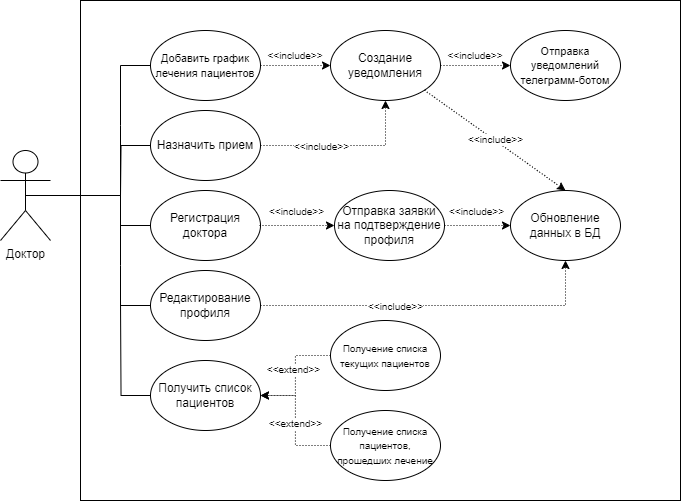
\includegraphics{pics/UML/Doctor.png}}
            \caption{Диаграмма прецедентов для роли "Доктор".} \label{doctor_uml}
        \end{figure} 
    
    \section{Диаграмма прецедентов для сущности "Менеджер"\ }
        Сущность "Менеджер”\ имеет следующие возможности:

        \begin{enumerate}
            \item Получение отзывов о врачах: Эта возможность позволяет менеджеру %
            просмотреть статистику доктора, такую как количество принятых пациентов, %
            проведенных консультаций, выписанных рецептов и других показателей, которые %
            могут помочь оценить эффективность работы доктора. Менеджер может использовать %
            эту информацию для анализа производительности доктора, определения его сильных и %
            слабых сторон, а также для принятия решений о его дальнейшем развитии и обучении. %
            Эта функция также может быть полезна для определения потребностей пациентов и %
            улучшения качества медицинских услуг, предоставляемых клиникой;
            \item Администрирование данных о врачах: Эта возможность позволяет%
             менеджеру подтверждать, отклонять заявку о регистрации доктора, %
             а также, при необходимости, отстранять доктора от врачебной деятельности. %
             Все это влечет за собой обновление данных в БД;
            \item Изменение данных пользователя. Это возможность позволяет менеджеру %
            редактировать данные пациента, которые были указаны при регистрации. %
            При изменении данных пользователя, система автоматически сохраняет новые %
            значения в базе данных, чтобы они были доступны для системных процессов, %
            которые могут нуждаться в этой информации;
        \end{enumerate}
    
        Итоговая диаграмма прецедентов изображена на рисунке \ref{manager_uml}.

        \begin{figure}[H]%current location
            \centering
            \scalebox{0.70}{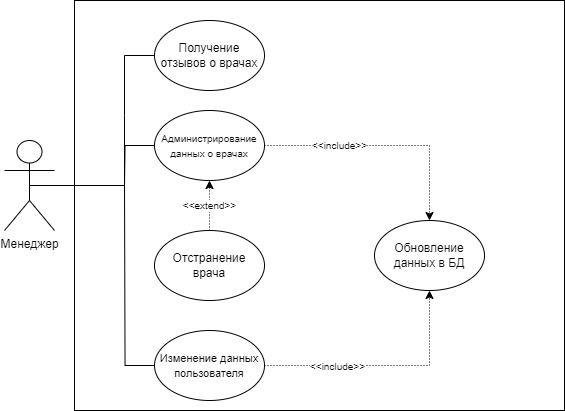
\includegraphics{pics/UML/Manager.png}}
            \caption{Диаграмма прецедентов для роли "Менеджер".} \label{manager_uml}
        \end{figure} 

\chapter{Проектирование базы данных приложения}

        В данной главе будет представлен процесс проектирования базы данных %
        веб-приложения для составления графика лечения на основании рекомендаций %
        врача.
        
    \section{Потенциальные объекты системы}
        В процессе анализа предметной области были выделены следующие примерные %
        бизнес-сущности, которые должны быть отображены в базе данных:

        \begin{itemize}
            \item Доктор;
            \item Пациент;
            \item Менеджер;
            \item Прием лекарств;
            \item Прием врача;
            \item Лекарственное средство;
            \item Рекомендации;
            \item Отзыв;
        \end{itemize}

    \section{Определение атрибутов и первичных ключей}

        Для оптимизации работы веб-приложения, было принято решение о %
        нормализации базы данных, объединив объекты системы в сущность "Пользователь". %
        Для реализации контроля доступа внутри системы будет введен атрибут роли, %
        который будет ограничивать доступ к изменению и получения данных из системы. %

        В таблице \ref{user-attrs-table} продемонстрированы атрибуты сущности "Пользователь".

        \begin{table}[H]
            \caption{Описание атрибутов сущности "Пользователь".}
            \label{user-attrs-table}
            \resizebox{\columnwidth}{!}{%
            \begin{tabular}{|p{0.225\linewidth}|p{0.3\linewidth}|p{0.2\linewidth}|p{0.2\linewidth}|}
            \hline
            Название атрибута & Обязательный/не обязательный (*/o) & Уникальный идентификатор (\#) & Тип для логической модели \\
            \hline
            idUser & * & \# & Числовой \\
            \hline
            email & * & (\#) & Символьный \\
            \hline
            role & * & & Символьный \\
            \hline
            firstName & * & & Символьный \\
            \hline
            secondName & * & & Символьный \\
            \hline
            lastName & & & Символьный \\
            \hline
            phoneNumber & & & Символьный \\
            \hline
            idTelegram & & & Числовой \\
            \hline
            idLicense & & & Символьный \\
            \hline
            isConfirmed & & & Логический \\
            \hline
            \end{tabular}%
            }
        \end{table}

        Поле "idTelegram"\ необходимо для авторации и рассылки уведомлений через %
        телеграмм-бота, который будет напоминать врачам и пользователям о изменении их %
        лечебного плана и напоминаний о приеме необходимых лекарственных препаратов. 

        Поля "idLicense"\ и "isConfirmed"\ относятся к роли врача. "idLicense"\ %
        относиться к номеру идентифицирующему документ об образовании врача. %
        Поле "isConfirmed"\ показывает был ли допущен к работе с пациентами после %
        проверки документов менеджером. 

    \newpage

    Взаимодействие между пациентои и доктором реализуется при помощи сущности пересечения, %
    которая показывает какие врачи производят наблюдения и рекомендации по лечебному плану для %
    определенного пользователя.

    В таблице \ref{patient-doctor-table} представлена сущность пересечения между %
    ролями системы "Пациент"\ и "Доктор".
    \newline
    \begin{table}[H]
        \caption{Описание атрибутов сущности пересечения ролей  "Пациент"\ и "Доктор".}
        \label{patient-doctor-table}
        \resizebox{\columnwidth}{!}{%
        \begin{tabular}{|p{0.225\linewidth}|p{0.3\linewidth}|p{0.2\linewidth}|p{0.2\linewidth}|}
        \hline
        Название атрибута & Обязательный/не обязательный (*/o) & Уникальный идентификатор (\#) & Тип для логической модели \\
        \hline
        idUser & * & \# & Числовой \\
        \hline
        idDoctor & * & \# & Числовой \\ 
        \hline
        \end{tabular}%
        }
    \end{table}

    Для реализации нотификаций, была выделена сущность "Прием лекарств". %
    Данная сущность дожна хранить в себе атрибуты, для следующих видов приема:
    
    \begin{itemize}
        \item Прием только один день;
        \item Ежедневный прем;
        \item Прием каждые X дней;
        \item Прием по конкретным датам;
        \item Цикл приема из X дней и Y дней пропуска; 
        \item Прием через определенный промежуток времени;
    \end{itemize}

    Также необходимо хранить необхдимое время приема в течении дня для повышения %
    эффективности лечения.

    В таблице \ref{pills-table} предоставлены атрибуты сущности "Прием лекарств".
    \newline

    \begin{table}[H]
        \caption{Описание атрибутов сущности "Прием лекарств".}
        \label{pills-table}
        \resizebox{\columnwidth}{!}{%
        \begin{tabular}{|p{0.225\linewidth}|p{0.3\linewidth}|p{0.2\linewidth}|p{0.2\linewidth}|}
        \hline
        Название атрибута & Обязательный/не обязательный (*/o) & Уникальный идентификатор (\#) & Тип для логической модели \\
        \hline
        idPill & * & \# & Числовой \\
        \hline
        idUser & * &  & Числовой \\
        \hline
        type & * & & Символьный \\
        \hline
        name & * & & Символьный \\
        \hline
        form & & & Символьный \\
        \hline
        note & & & Симовльный \\
        \hline
        startDate & * & & Даты и времени \\
        \hline
        endDate & & & Даты и времени \\
        \hline
        time & & & Временной \\
        \hline
        days & & & Дата \\
        \hline
        deltaTakeDays & & & Числовой \\
        \hline
        deltaPassDays & & & Числовой \\
        \hline
        timeDelta & & & Временной \\
        \hline
        lastNotify & & & Даты и времени \\ 
        \hline
        \end{tabular}%
        }
    \end{table}
    
    Для отслеживание удовлетворенности пользвателей в услугах выбранного лечащего %
    врача была введена сущность "Отзыв". Данная сущность предназначена для администрирования %
    площадки менеджером и отслеживании качества предоставляемых докторами услуг.

    Атрибуты сущности "Отзыв"\ предоставлены в таблице \ref{comment-table}

    \begin{table}[H]
        \caption{Описание атрибутов сущности "Отзыв".}
        \label{comment-table}
        \resizebox{\columnwidth}{!}{%
        \begin{tabular}{|p{0.225\linewidth}|p{0.3\linewidth}|p{0.2\linewidth}|p{0.2\linewidth}|}
        \hline
        Название атрибута & Обязательный/не обязательный (*/o) & Уникальный идентификатор (\#) & Тип для логической модели \\
        \hline
        idComment & * & \# & Числовой \\
        \hline
        idPatient & * &  & Числовой \\
        \hline
        idDoctor & * & & Числовой \\
        \hline
        rate & * & & Числовой \\
        \hline
        review & & & Символьный \\
        \hline

        \end{tabular}%
        }
    \end{table}

    Для эффективного процесса лечения также необходимы своевременное посещение %
    лечащего врача. Для этого в системе необходимо хранить информацию о плановых посещениях, %
    которые представлены в сущности "Прем врача".

    В таблице \ref{visit-table} продемонстрированы атрибуты сущности "Прием врача".

    \begin{table}[H]
        \caption{Описание атрибутов сущности "Отзыв".}
        \label{visit-table}
        \resizebox{\columnwidth}{!}{%
        \begin{tabular}{|p{0.225\linewidth}|p{0.3\linewidth}|p{0.2\linewidth}|p{0.2\linewidth}|}
        \hline
        Название атрибута & Обязательный/не обязательный (*/o) & Уникальный идентификатор (\#) & Тип для логической модели \\
        \hline
        idVisit & * & \# & Числовой \\
        \hline
        idPatient & * &  & Числовой \\
        \hline
        idDoctor & & & Числовой \\
        \hline
        appointmentTime & * & & Даты и времени \\
        \hline
        note & & & Символьный \\
        \hline
        \end{tabular}%
        }
    \end{table}
    
    Для предоставления комфортного пользования сервисом были выделены справочные сущности, %
    которые позволяют пользователю ознакомиться с препаратами и предоставить поддержку советами %
    о правильном лечении.

    Сущность "Лекарственное средство"\ является справочной сущностью возможных %
    лекартсвенных препаратов. Аттрибуты данной сущности продемонстрированы в %
    таблице \ref{pills-type-table}

    \begin{table}[H]
        \caption{Описание атрибутов сущности "Отзыв".}
        \label{comment-table}
        \resizebox{\columnwidth}{!}{%
        \begin{tabular}{|p{0.225\linewidth}|p{0.3\linewidth}|p{0.2\linewidth}|p{0.2\linewidth}|}
        \hline
        Название атрибута & Обязательный/не обязательный (*/o) & Уникальный идентификатор (\#) & Тип для логической модели \\
        \hline
        idPillType & * & \# & Числовой \\
        \hline
        name & * &  & Символьный \\
        \hline
        dose & * & & Числовой \\
        \hline
        form & * & & Символьный \\
        \hline
        description & & & Символьный \\
        \hline
        \end{tabular}%
        }
    \end{table}

    Сущность "Совет"\ является справочной сущностью, которая должна помочь пользователю %
    придерживаться эффективного плана лечения. Атрибуты сущности "Совет"\ предоставлены в %
    таблице \ref{tips-table}.
    
    \begin{table}[H]
        \caption{Описание атрибутов сущности "Отзыв".}
        \label{tips-table}
        \resizebox{\columnwidth}{!}{%
        \begin{tabular}{|p{0.225\linewidth}|p{0.3\linewidth}|p{0.2\linewidth}|p{0.2\linewidth}|}
        \hline
        Название атрибута & Обязательный/не обязательный (*/o) & Уникальный идентификатор (\#) & Тип для логической модели \\
        \hline
        idTips & * & \# & Числовой \\
        \hline
        title & * &  & Символьный \\
        \hline
        content & * & & Символьный \\
        \hline
        \end{tabular}%
        }
    \end{table}

    \section{Логическое проектирование базы данных}
        Логическое проектирование базы данных веб-прилоежения было произведено %
        при помощи программы "PgAdmin" \cite{pg-admin}. Данный комплекс программного обеспечения %
        является мощным инструментом для логического проектирования и %
        администрирования баз данных. Оно предоставляет возможность %
        создания ERD (Entity-Relationship Diagram) диаграмм, которые %
        представляют структуру базы данных и связи между ее элементами.
        "PgAdmin"\ также позволяет конвертировать ERD диаграммы в %
        SQL-скрипты, которые можно использовать для создания таблиц в %
        базе данных. Это значительно упрощает процесс разработки, так как %
        позволяет автоматически генерировать SQL-скрипты на основе диаграммы. %
        Результат преобразования сущностей в ERD диаграму изображен на рисунке \ref{erd_diagram}.

        \newpage
        \begin{landscape}
            \begin{figure}[H]%current location
                \centering
                \scalebox{0.42}{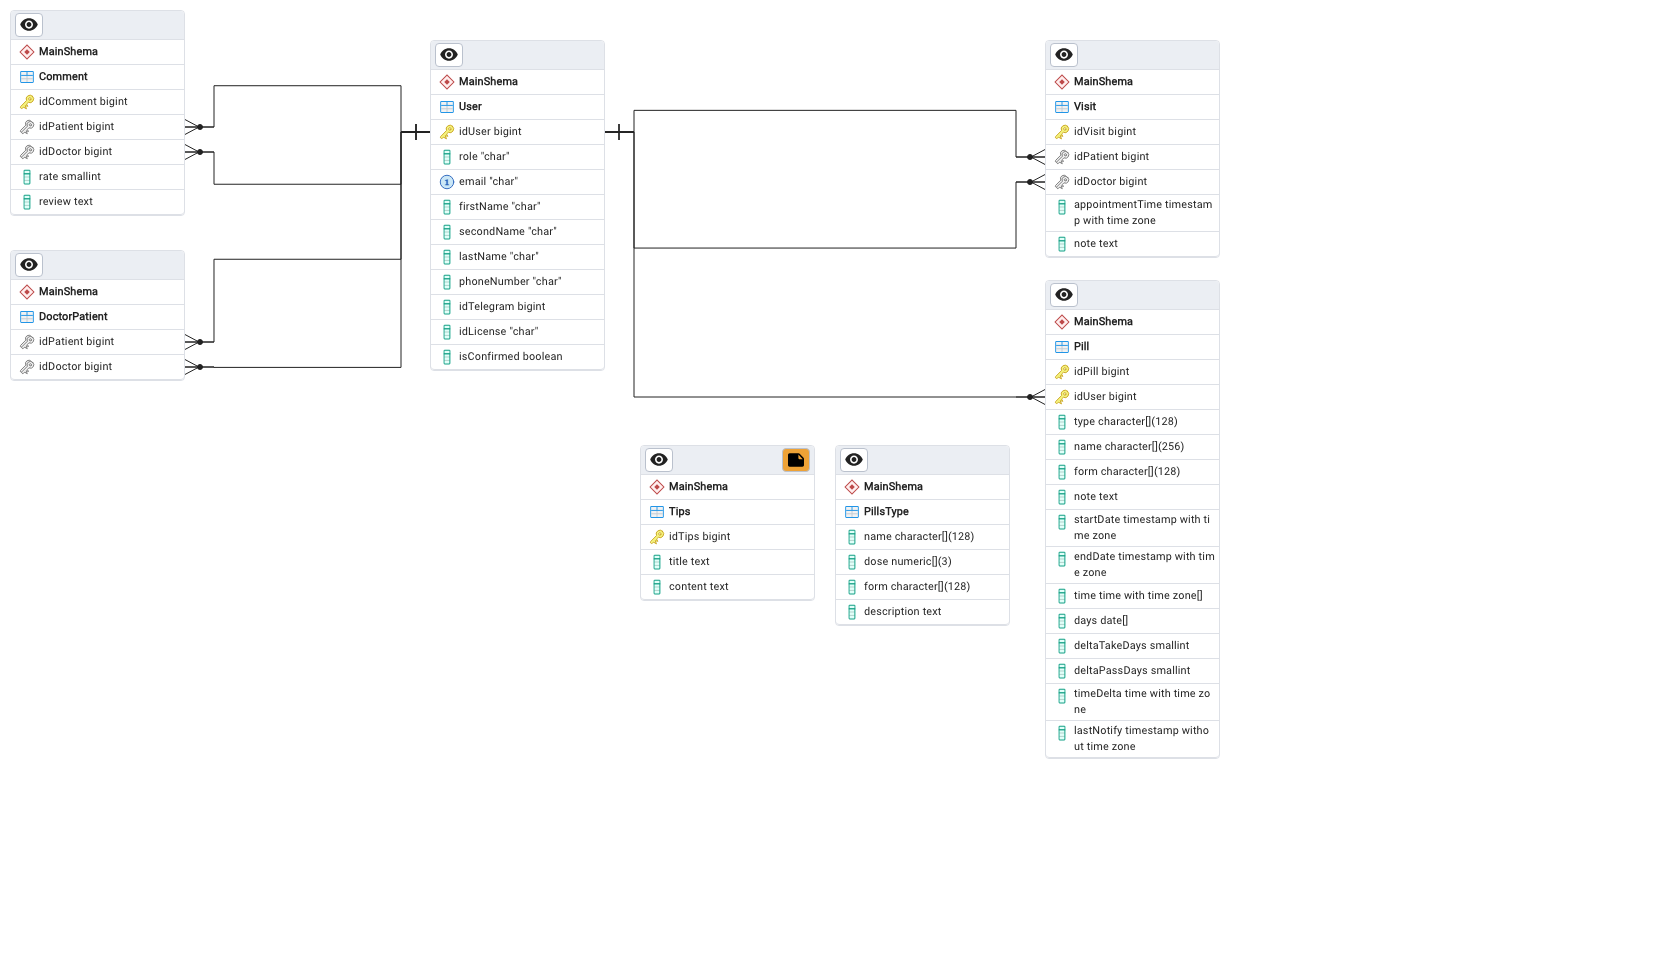
\includegraphics{pics/database/ERR-diagram.png}}
                \caption{ERD диаграмма базы данных.} \label{erd_diagram}
            \end{figure} 

        \end{landscape}

\chapter{Алгоритмы работы с пользователем}

    В данном разделе будут представлены алгоритмы работы с потенциальным пользователем %
    веб-приложения.

    \section{Диаграммы активности}
        Диаграмма активности  “Регистрация пациента”\ представляет %
        собой последовательность следующих действий:
        \begin{enumerate}
            \item Пользователь отправляет данные для регистрации;
            \item Происходит проверка данных на валидность, в случае не %
            валидности данных пользователь вводит данные снова, а в %
            случае валидности - происходит следующая проверка;
            \item Происходит проверка на уникальность пациента, в %
            случае не уникальности пациента - пользователь вводит данные %
            снова, в ином случае - происходит регистрация пользователя;
        \end{enumerate}

        Диаграмма активности “Регистрация пациента” изобрaжена на рисунке \ref{diagram-registration}.
        \begin{figure}[H]%current location
            \centering
            \scalebox{0.42}{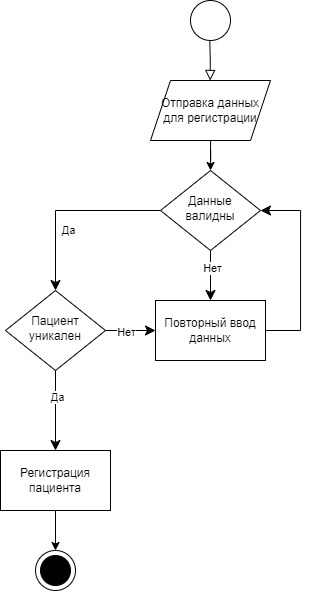
\includegraphics{pics/diagrams/register.png}}
            \caption{Диаграмма активности “Регистрация пациента”.} \label{diagram-registration}
        \end{figure} 

        Диаграмма активности  “Получить список пациентов” представляет собой %
        последовательность следующих действий:

        \begin{itemize}
            \item Пользователь отправляет запрос на получение списка пациентов;
            \item Происходит проверка на существование данных, в случае %
            существовании данных происходит следующий этап - получение списка %
            пациентов, в ином случае - происходит извещение доктора об отсутствии пациентов;
        \end{itemize}
        
        Диаграмма активности  “Получить список пациентов” изобрaжена на рисунке \ref{diagram-patient-list}.

        \begin{figure}[H]%current location
            \centering
            \scalebox{0.6}{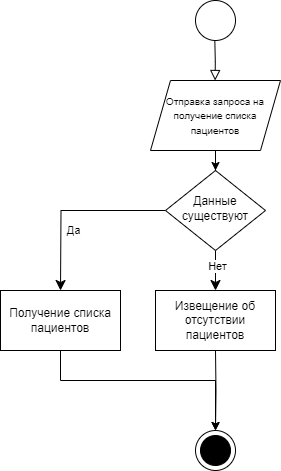
\includegraphics{pics/diagrams/patient-list.png}}
            \caption{Диаграмма активности  “Получить список пациентов”.} \label{diagram-patient-list}
        \end{figure} 

        Диаграмма активности “Администрирование данных о врачах” %
        представляет собой последовательность следующих действий:
        \begin{enumerate}
            \item Менеджер отправляет запрос на получение данных о врачах;
            \item Происходит проверка корректности данных, если данные %
            корректны, то происходит следующий этап, в ином случае происходит %
            отказ в доступе к пациентам для врача;
            \item Происходит проверка на приемлемость отзывов лечащего врача, %
            оставленных пациентами, в случае, если отзывы приемлемы врач %
            утверждается, в ином случае - происходит отказ в доступе к пациентам %
            для врача;
        \end{enumerate}
        
        Диаграмма активности “Администрирование данных о врачах” изображена %
        на рисунке \ref{diagram-doctor-admin}.
        \begin{figure}[H]%current location
            \centering
            \scalebox{0.6}{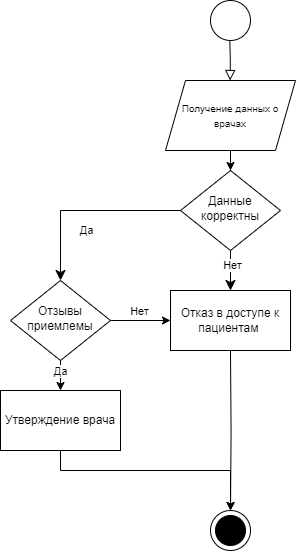
\includegraphics{pics/diagrams/doctor-admin.png}}
            \caption{Диаграмма активности “Администрирование данных о врачах”.} \label{diagram-doctor-admin}
        \end{figure} 
    
    \section{Контекстные диаграммы взаимодейсвия}
        В данном подразделе представлена модель в стандарте IDEF3, которая %
        описывает информационные потоки и взаимоотношения между процессами %
        обработки информации и объектами, являющимися частью этих процессов. %
        Модель представлена в виде контекстной диаграммы (рисунок \ref{context-diagram}), которая %
        представляет собой графическое представление основных компонентов системы и %
        их взаимосвязей и позволяет определить основные процессы и объекты, которые %
        участвуют в обработке информации, а также информационные потоки между ними. %
        
        \begin{figure}[H]%current location
            \centering
            \scalebox{0.6}{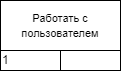
\includegraphics{pics/IDEF3/context-diagram.png}}
            \caption{Контекстная диаграмма (IDEF3)} \label{context-diagram}
        \end{figure} 
        
        Декомпозиции этой диаграммы изобажена на рисунке \ref{context-decomposition}. %
        Декомпозиция представляет собой более детальное %
        представление процессов и объектов, описанных в контекстной диаграмме, позволяет %
        более подробно описать каждый процесс и объект, а также их взаимосвязи. кроме того, %
        она включает в себя описание входных и выходных данных, используемых ресурсов, %
        исполнителей, необходимых для выполнения процессов.


        \begin{landscape}
            \begin{figure}[H]%current location
                \centering
                \scalebox{0.4}{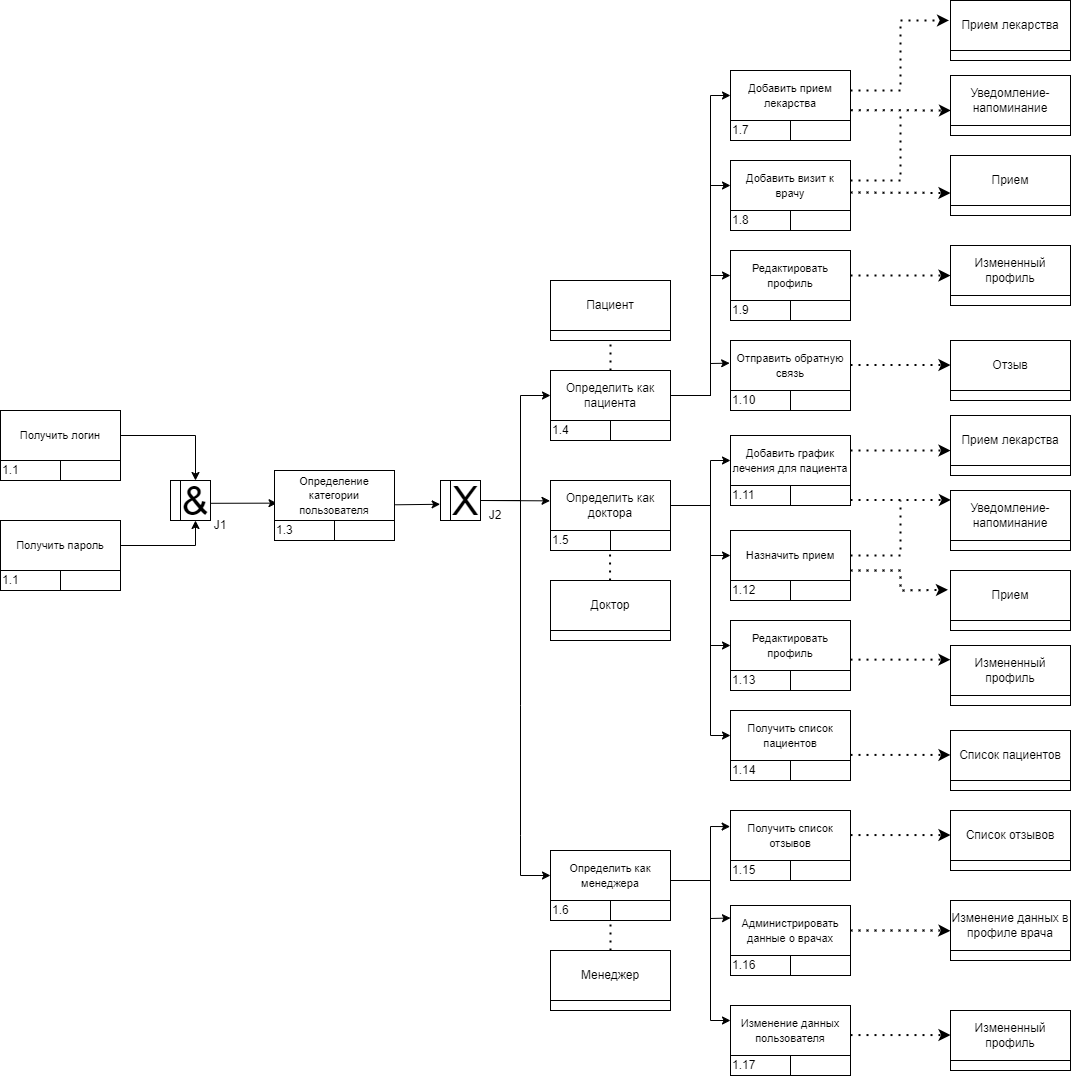
\includegraphics{pics/IDEF3/context-decomposition.png}}
                \caption{Декомпозиция контекстной диаграммы} \label{context-decomposition}
            \end{figure} 
        \end{landscape}

        Декомпозиции блока “Администрировать данные о врачах” представлена на рисунке \ref{context-doctor-admin}

        \begin{figure}[H]%current location
            \centering
            \scalebox{0.5}{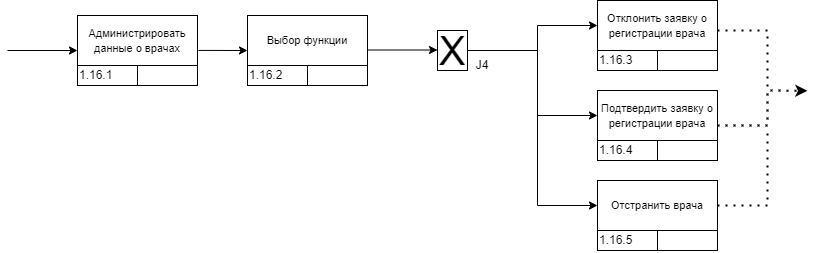
\includegraphics{pics/IDEF3/context-doctor-admin.png}}
            \caption{Декомпозиции блока “Администрировать данные о врачах”} \label{context-doctor-admin}
        \end{figure} 

        Декомпозиция блока Декомпозиция блока “Получить список пациентов” представлена на рисунке \ref{context-patient-list}

        \begin{figure}[H]%current location
            \centering
            \scalebox{0.5}{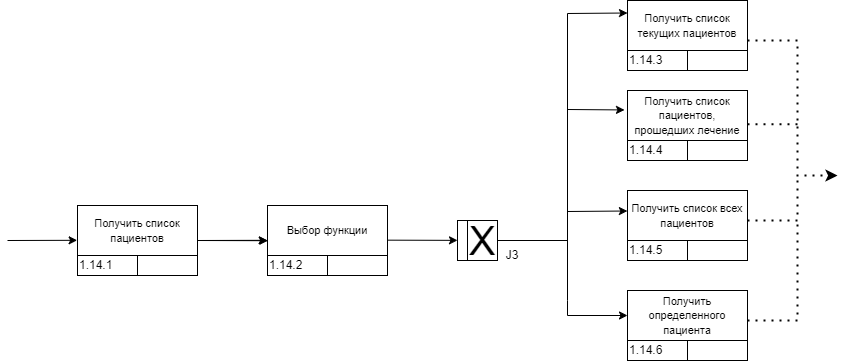
\includegraphics{pics/IDEF3/context-user-list.png}}
            \caption{Декомпозиции блока “Администрировать данные о врачах”} \label{context-patient-list}
        \end{figure} 
        
        Декомпозиция блока “Редактировать профиль” представлена на рисунке \ref{context-change-profile}

        \begin{figure}[H]%current location
            \centering
            \scalebox{0.5}{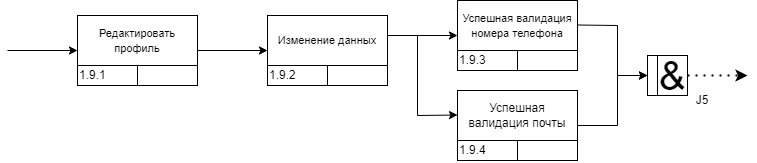
\includegraphics{pics/IDEF3/context-change-profile.png}}
            \caption{Декомпозиции блока “Администрировать данные о врачах”} \label{context-change-profile}
        \end{figure} 


\chapter{Технологии программирования}
    В данной главе будут представлены выбранные технологии программироания %
    которые будут применены при разработке веб-приложения для составления %
    графика лечения на основании рекомендаций врача.

    \section{Веб-приложение}
        Для реализации клиент-серверной архитектуры будут применяться %
        следующие технологии программирования:
        \begin{enumerate}
            \item Django \cite{django} - это обширная библеотека для %
            языка Python, которая предоставляет множество инструментов для %
            разработки веб-приложений. Она обеспечивает высокую производительность, %
            безопасность и масштабируемость. Django также имеет встроенную поддержку %
            для работы с базами данных, шаблонизации и аутентификации.
            \item React \cite{react} - это библиотека для создания пользовательских %
            интерфейсов на языке JavaScript. Она предоставляет мощные инструменты %
            для создания интерактивных и высокопроизводительных веб-приложений. %
            React позволяет легко управлять состоянием приложения и обновлять %
            его части, что делает его идеальным выбором для разработки %
            сложных интерфейсов.
        \end{enumerate}
    
    \section{Система уведомлений пользователей}
        Для реализации системы уведомлений пользователей было принято решение %
        воспользоваться телеграмм-ботом для рассылки уведомлений. Данный выборс связан %
        с обширной базой пользователей телеграма\cite{telegram}. Потому что, как правило, %
        у потенциальных пользователей данный меснджер установлен на всех основных устройствах.

        Для программной реализации данной концепции была выбрана библеотека Aiotelegram \cite{aiotelegram} %
        Данная библиотека предназначена для работы с интерфейс программирования приложения (API) Telegram. Она позволяет %
        разработчикам создавать ботов для Telegram и создавать интерактивные пути взаимодействия с пользователем. В данном %
        случае будет создан телеграмм-бот для отправки уведомлений пациентам.
    
    \section{Развертывание приложения}
        Для успешной эксплуатации приложения, планируется использовать современные технологии %
        развертывания приложений. В достижении гибкости использования предоставленной провайдером %
        серверной архитектуры будет использоваться инструмент контейнеризации приложений под названием %
        Docker \cite{docker}. Так как приложения является небольшим, то для оркестрации данных контейнеров будет использоваться %
        поставляемый вместе с Docker инструмент Docker-compose \cite{docker-compose}.
        Использование данного подхода технологий позволит создать надежное и %
        масштабируемое веб-приложение для составления графика лечения на %
        основании рекомендаций врача. 
        

% Оформляем библиографию в соответствии с ГОСТ 7.0.5
% \bibliographystyle{ugost2008}
% если хотим включить все источники из библиографии даже не имеющие ссылки из текта
% \nocite{*}
% файл с библиографией
% \bibliography{biblio.bib}

\newpage
    \begin{thebibliography}{99}
        \bibitem{internet_users} Аудитория интернета в 2022 году.: %
        MediaScope [Электронный ресурс]. - 2023. - URL: %
        \url{https://mediascope.net/upload/iblock/3d8/qrlhud7t7dxyzw1rhtzxg3rwk8deg7uk/2022_ИНТЕРНЕТ.pdf} %
        (дата обращения 10.02.2023)

        \bibitem{diagrams_dot_net} diagrams.net.: Официальный сайт. - %
        URL: \url{https://vk.com/wall-132685896_980} (дата обращения 10.02.2023)

        \bibitem{django} Django.: Официальный сайт. - %
        URL: \url{https://www.djangoproject.com} (дата обращения 10.02.2023) 
        \bibitem{react} React.: Официальный сайт. - %
        URL: \url{https://ru.legacy.reactjs.org} (дата обращения 10.02.2023) 
        \bibitem{telegram} Telegram.: Официальный сайт. - %
        URL: \url{https://telegram.org} (дата обращения 10.02.2023) 
        \bibitem{aiotelegram} aiogram.: Официальный сайт. - %
        URL: \url{https://aiogram.dev} (дата обращения 10.02.2023) 
        \bibitem{docker} Docker.: Официальный сайт. - %
        URL: \url{https://www.docker.com} (дата обращения 10.02.2023) 
        \bibitem{docker-compose} Docker.: Официальный сайт. - %
        URL: \url{https://docs.docker.com/compose/} (дата обращения 10.02.2023) 

    \end{thebibliography}



\end{document}